\beginsong{Die Lappen Hoch}[
    wuw={Jurij Andreev, Nerother Wandervogel}, 
    jahr={1954},
    bo={78}, 
    pfii={38}, 
    pfiii={17}, 
    gruen={160}, 
    kssiv={60}, 
    siru={54},
]

\beginverse
\endverse
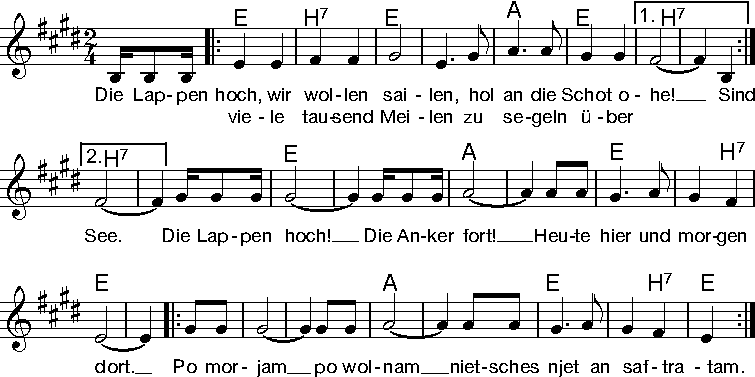
\includegraphics[draft=false, width=1\textwidth]{Noten/Lied024.pdf}

\beginverse
Wenn \[E]einst am La\[H7]gunen\[E]rande in \[A]Lee liegt \[E]unser \[H7]Boot,
Lacht \[E]uns das \[H7]Glück am \[E]Strande, am \[A]Strande \[E]gelb und \[H7]rot.
\endverse

\beginchorus
Die Lappen \[E]hoch, die Anker \[A]fort, heute \[E]hier und \[H7]morgen \[E]dort.
Po morjam, po wol\[A]nam nietsches \[E]njet an \[H7]Safra\[E]tam.
\endchorus

\beginverse
Und nie ^würdest ^weiter du ^ziehen und ^ewig ^bliebest du ^dann,
Ja, ^wenn nicht ^wäre das ^Segeln, der ^Wind und der ^Oze^an.
\endverse

\printchorus

\endsong

\beginscripture{}
''Po morjam...'' bedeutet: Auf's Meer, auf die Wellen, heute hier und morgen dort!
\endscripture
